\documentclass[11pt]{article}

\usepackage[a4paper,margin=1in]{geometry}
\usepackage{graphicx}
\usepackage{subcaption}
\usepackage{booktabs}
\usepackage{float}
\usepackage{amsmath,amssymb}
\usepackage{hyperref}
\usepackage{xcolor}

\hypersetup{
  colorlinks=true,
  linkcolor=blue!60!black,
  citecolor=blue!60!black,
  urlcolor=blue!60!black
}

\title{Latent-Key Associative Recall in Causal Transformers}
\author{Empirical Report}
\date{August 10, 2026}

\begin{document}
\maketitle

\begin{abstract}
This report summarizes the current small-scale Latent-Key Associative Recall experiments.
The goal is to test whether a causal Transformer can combine two kinds of memory:
a persistent parametric address map \(Q \mapsto K^\star\), and an episode-specific in-context dictionary \(K \mapsto V\).
The completed results show that one-layer attention fails, two-layer attention succeeds, embedding-only training fails, fixed embeddings still allow learning, attention-only training succeeds, and freezing QK mostly destroys performance. These results suggest that the main learned associative-memory mechanism is not merely the embedding table; it lives in the trainable attention pathway, with QK playing a necessary addressing role and V/O/output pathways needed for value copying.
\end{abstract}

\section{Task Definition}

The experiment uses three disjoint token sets:
\[
\mathcal Q = [N_Q], \qquad
\mathcal K = [N_K], \qquad
\mathcal V = [N_V].
\]
At the beginning of an experimental run, we sample one fixed ground-truth memory:
\[
\pi_\star: \mathcal Q \to \mathcal K.
\]
In the current experiments, \(\pi_\star\) is a random query-to-key assignment and remains fixed throughout training and evaluation.

Each training episode samples a query \(q\), usually from a Zipf distribution.
The correct latent key is
\[
K^\star = \pi_\star(q).
\]
The episode then builds a candidate key set \(S\) of size \(m\), containing the correct key and \(m-1\) decoy keys:
\[
S = \{K^\star, K_2, \ldots, K_m\}.
\]
For this episode only, we sample a fresh injective value assignment:
\[
g_e: S \to \mathcal V.
\]
The target value is therefore
\[
V^\star = g_e(\pi_\star(q)).
\]

The crucial design choice is that \(g_e\) is resampled independently in every episode.
Therefore the model cannot memorize a direct map \(Q \mapsto V\).
It must learn the persistent address map \(Q \mapsto K^\star\), and then use the current context to retrieve \(K^\star \mapsto V^\star\).

\section{Sequence Generation}

Each example is a standard causal next-token prediction sequence.
The prompt has the form
\[
[\mathrm{BOS}], [K_1], [V_1], \ldots, [K_m], [V_m], [\mathrm{noise}], [Q],
\]
and the model is trained to predict the next token
\[
[V^\star].
\]

In words, each sequence contains:
\begin{itemize}
  \item one beginning-of-sequence token;
  \item \(m\) key-value pairs;
  \item optional noise tokens inserted between pairs or before the query;
  \item one query token at the end;
  \item one answer token, used only as the training target.
\end{itemize}

For the main completed architecture study:
\[
N_Q=N_K=128,\qquad N_V=512,\qquad m=7.
\]
Thus the random candidate baseline is
\[
\frac{1}{m} = \frac{1}{7} \approx 14.3\%.
\]
The sequence length sweep is
\[
L \in \{16,32,64\},
\]
and the model dimension sweep is
\[
d_{\mathrm{model}} \in \{64,128,256\}.
\]

The training objective is answer-token next-token cross entropy:
\[
\mathcal L(\theta)
=
-\log p_\theta
\left(
V^\star
\mid
[\mathrm{BOS}], K_1,V_1,\ldots,K_m,V_m,\mathrm{noise},Q
\right).
\]

\section{Metrics}

We track the following metrics.

\paragraph{Candidate accuracy.}
The model is evaluated only among the \(m\) candidate values appearing in the current context.
This measures whether the model selected the correct in-context value.

\paragraph{Full-vocabulary accuracy.}
The model is evaluated over the entire vocabulary.
This is stricter and corresponds to true next-token top-1 accuracy.

\paragraph{Loss.}
Answer-token cross entropy.

\paragraph{Candidate margin.}
The correct candidate value logit minus the largest decoy candidate value logit:
\[
\mathrm{margin}
=
\ell(V^\star) - \max_{V \in g_e(S),\, V\neq V^\star} \ell(V).
\]

\paragraph{Head and tail accuracy.}
Queries are sorted by training frequency under the Zipf distribution.
Head accuracy is measured on the most frequent quartile, and tail accuracy on the rarest quartile.

\section{Architecture and Pathway Ablations}

The architecture study asks two questions:
\begin{enumerate}
  \item Which Transformer architectures can solve this task?
  \item Which parameter pathways carry the associative-memory computation?
\end{enumerate}

The following ablations were compared:
\begin{itemize}
  \item \textbf{1L-attn}: one attention-only Transformer block.
  \item \textbf{2L-attn}: two attention-only Transformer blocks.
  \item \textbf{2L-full}: two Transformer blocks with MLPs.
  \item \textbf{4L-full}: four Transformer blocks with MLPs.
  \item \textbf{2L-no-pos}: two attention-only blocks without position embeddings.
  \item \textbf{2L-fixed-embed}: token/position/output embeddings frozen; Transformer body trainable.
  \item \textbf{2L-embed-only}: only embeddings/output head trainable; Transformer body frozen.
  \item \textbf{2L-attn-only}: only attention matrices trainable.
  \item \textbf{2L-qk-only}: only Q and K projection matrices trainable.
  \item \textbf{2L-freeze-QK}: all trainable except Q and K projections.
\end{itemize}

All architecture/pathway runs use AdamW with learning rate \(10^{-3}\).
Each setting uses two seeds.

\begin{table}[H]
\centering
\caption{Architecture/pathway results at \(L=32\), \(d_{\mathrm{model}}=128\).}
\label{tab:arch-anchor}
\resizebox{\textwidth}{!}{
\begin{tabular}{lrrrrrr}
\toprule
Setting & Candidate Acc. & Full-Vocab Acc. & Loss & Margin & Head Acc. & Tail Acc.\\
\midrule
2L-attn & 0.9629 & 0.9629 & 0.1956 & 9.5691 & 0.9883 & 0.9375\\
2L-fixed-embed & 0.9365 & 0.9365 & 0.8900 & 5.6477 & 1.0000 & 0.8711\\
2L-attn-only & 0.9355 & 0.9355 & 4.4659 & 1.8510 & 0.9883 & 0.8516\\
2L-full & 0.5352 & 0.5293 & 2.0855 & 3.3109 & 0.5469 & 0.4688\\
2L-no-pos & 0.4238 & 0.4180 & 2.6085 & 0.0932 & 0.7773 & 0.1914\\
4L-full & 0.4150 & 0.3760 & 3.2549 & 0.4546 & 0.5156 & 0.3242\\
2L-embed-only & 0.1504 & 0.0498 & 5.2637 & -1.3435 & 0.1445 & 0.1641\\
2L-qk-only & 0.1416 & 0.0029 & 6.6650 & -0.3021 & 0.1563 & 0.1328\\
1L-attn & 0.1357 & 0.1357 & 3.1112 & -1.8881 & 0.1328 & 0.1328\\
2L-freeze-QK & 0.1221 & 0.1191 & 3.4723 & -2.0748 & 0.1445 & 0.1289\\
\bottomrule
\end{tabular}
}
\end{table}

\begin{figure}[H]
\centering
\begin{subfigure}{0.49\textwidth}
  \centering
  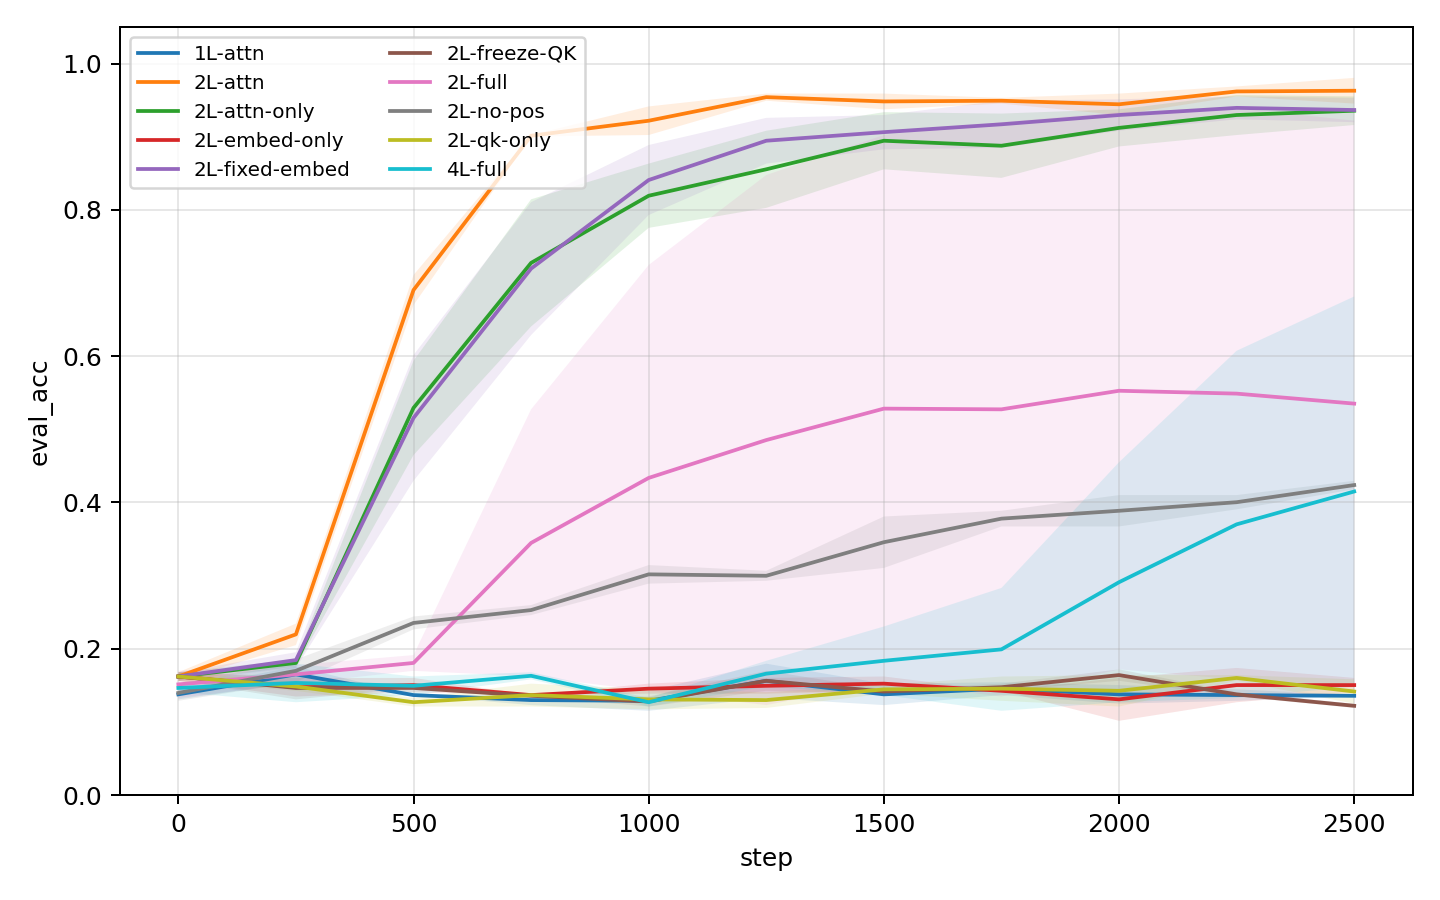
\includegraphics[width=\textwidth]{figures/architecture_curves_seq32_d128.png}
  \caption{Candidate accuracy}
\end{subfigure}
\begin{subfigure}{0.49\textwidth}
  \centering
  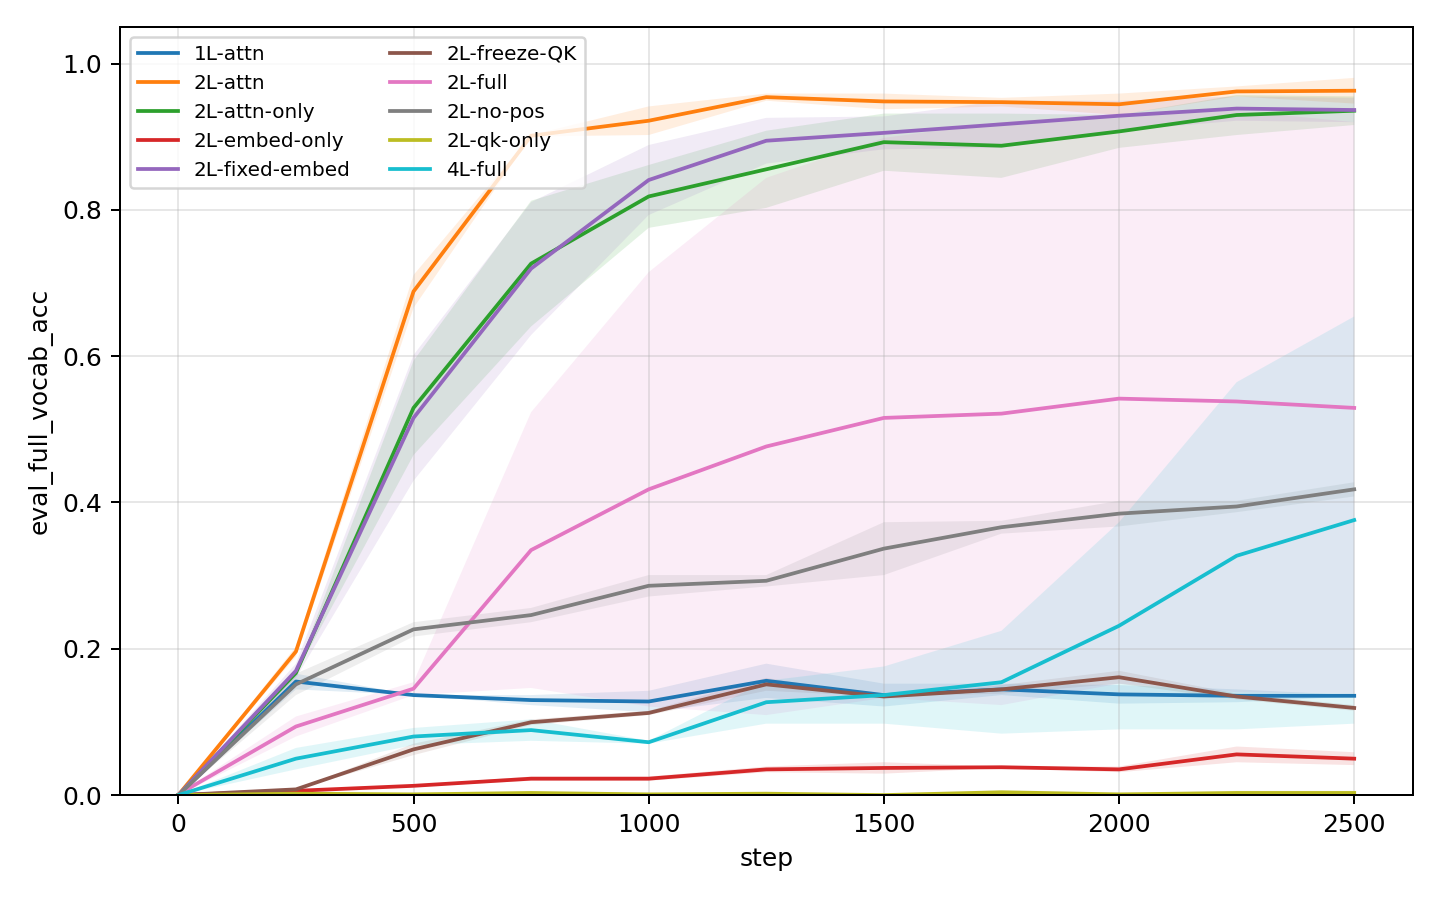
\includegraphics[width=\textwidth]{figures/architecture_full_vocab_curves_seq32_d128.png}
  \caption{Full-vocabulary accuracy}
\end{subfigure}
\caption{Architecture/pathway learning curves at \(L=32\), \(d_{\mathrm{model}}=128\). Curves show seed means; bands show SEM.}
\label{fig:arch-curves}
\end{figure}

\section{Architecture Results}

\paragraph{One layer is insufficient.}
The one-layer attention model stays near random baseline.
This matches the mechanistic expectation: when keys and values are separate adjacent tokens, the final query cannot easily attend to a value token by matching against the previous key in the same layer.

\paragraph{Two attention layers are sufficient.}
The two-layer attention-only model solves the task reliably.
This supports a two-stage computation:
the first layer binds each value position to its preceding key, and the second layer lets the query retrieve the correct bound value.

\paragraph{Embedding-only does not solve the task.}
The embedding-only ablation remains near random candidate accuracy and has very low full-vocabulary accuracy.
This argues against the hypothesis that the embedding table alone is memorizing the task.

\paragraph{Fixed embeddings still allow learning.}
The fixed-embedding model performs strongly.
Therefore, trainable embeddings are not necessary for solving the task.

\paragraph{Attention-only training is sufficient.}
The attention-only ablation also performs strongly.
This suggests that the learned associative-memory computation is mainly carried by the attention pathway.

\paragraph{QK is necessary but not sufficient.}
Freezing QK destroys performance, showing that trainable QK addressing is important.
However, QK-only training also fails.
This means that in a real Transformer, QK is not enough by itself: the model also needs value/output pathways to copy the selected value into the answer logit.

\section{Optimizer Comparison Results}

The optimizer study fixes the architecture to:
\[
\text{2L-attn},\qquad L=32,\qquad d_{\mathrm{model}}=128.
\]
It compares AdamW, Muon, NGD, and SGD over the same log-scale learning-rate grid.

\textbf{Important caveat.}
The completed optimizer sweep used global gradient clipping.
This makes the NGD versus SGD comparison confounded, because clipping can make ordinary SGD behave similarly to normalized gradient descent.

\begin{table}[H]
\centering
\caption{Optimizer pilot results: best over learning rate under the clipped protocol.}
\label{tab:opt}
\begin{tabular}{lrrrrrr}
\toprule
Optimizer & Best LR & Candidate Acc. & Full-Vocab Acc. & Loss & Margin & AUC\\
\midrule
AdamW & 0.0003 & 0.9805 & 0.9805 & 0.0751 & 9.7127 & 0.7179\\
Muon & 0.0010 & 0.9987 & 0.9987 & 0.0056 & 11.6486 & 0.7264\\
NGD & 0.0300 & 0.1576 & 0.0104 & 6.2060 & -0.2098 & 0.1463\\
SGD & 0.0300 & 0.1576 & 0.0104 & 6.2060 & -0.2098 & 0.1463\\
\bottomrule
\end{tabular}
\end{table}

\begin{figure}[H]
\centering
\begin{subfigure}{0.49\textwidth}
  \centering
  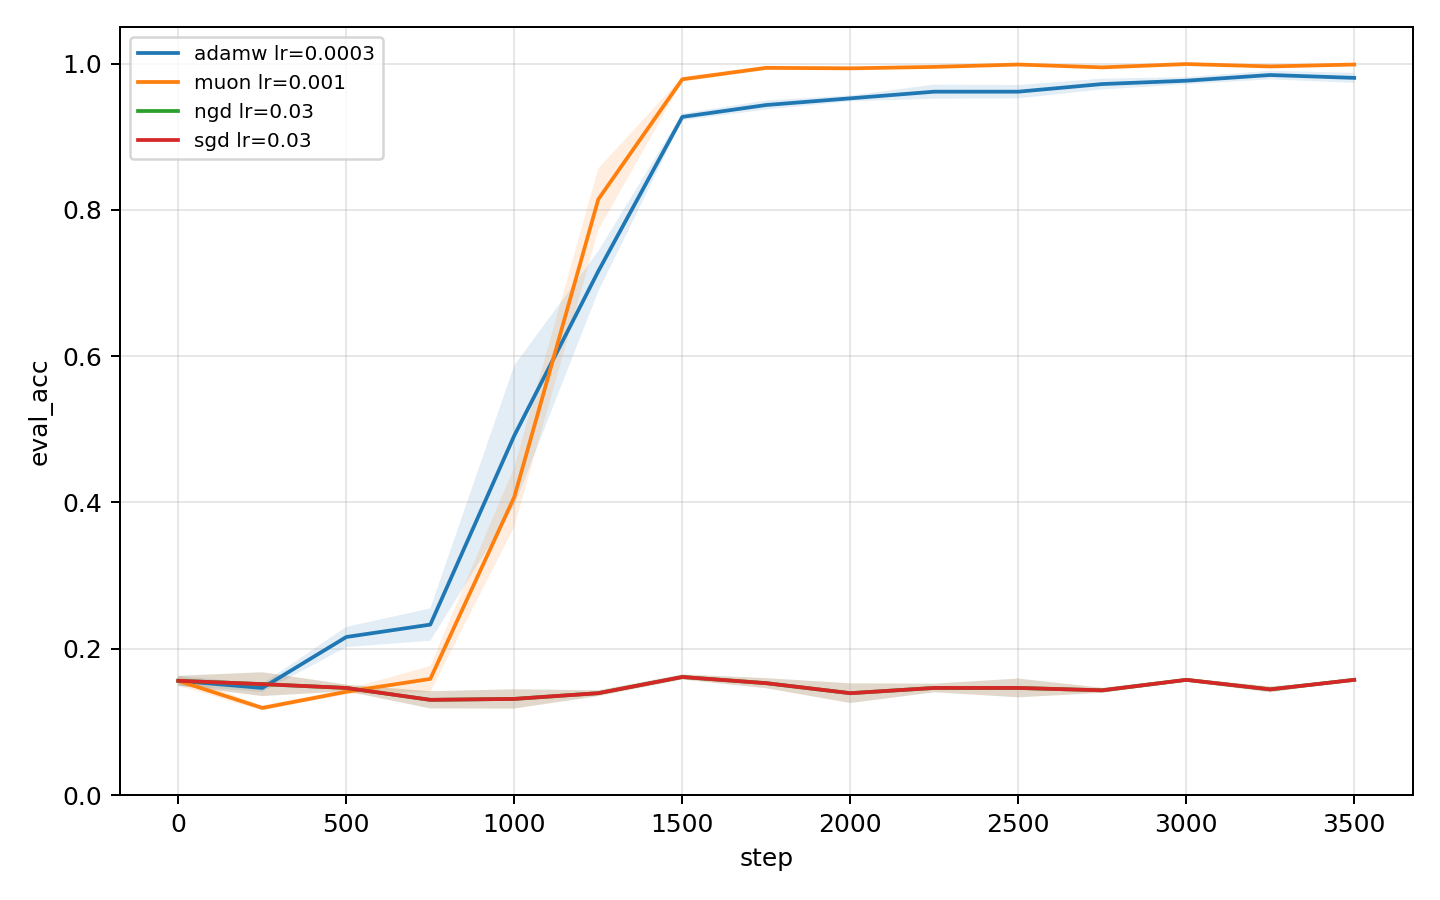
\includegraphics[width=\textwidth]{figures/optimizer_curves_best_lr.png}
  \caption{Candidate accuracy}
\end{subfigure}
\begin{subfigure}{0.49\textwidth}
  \centering
  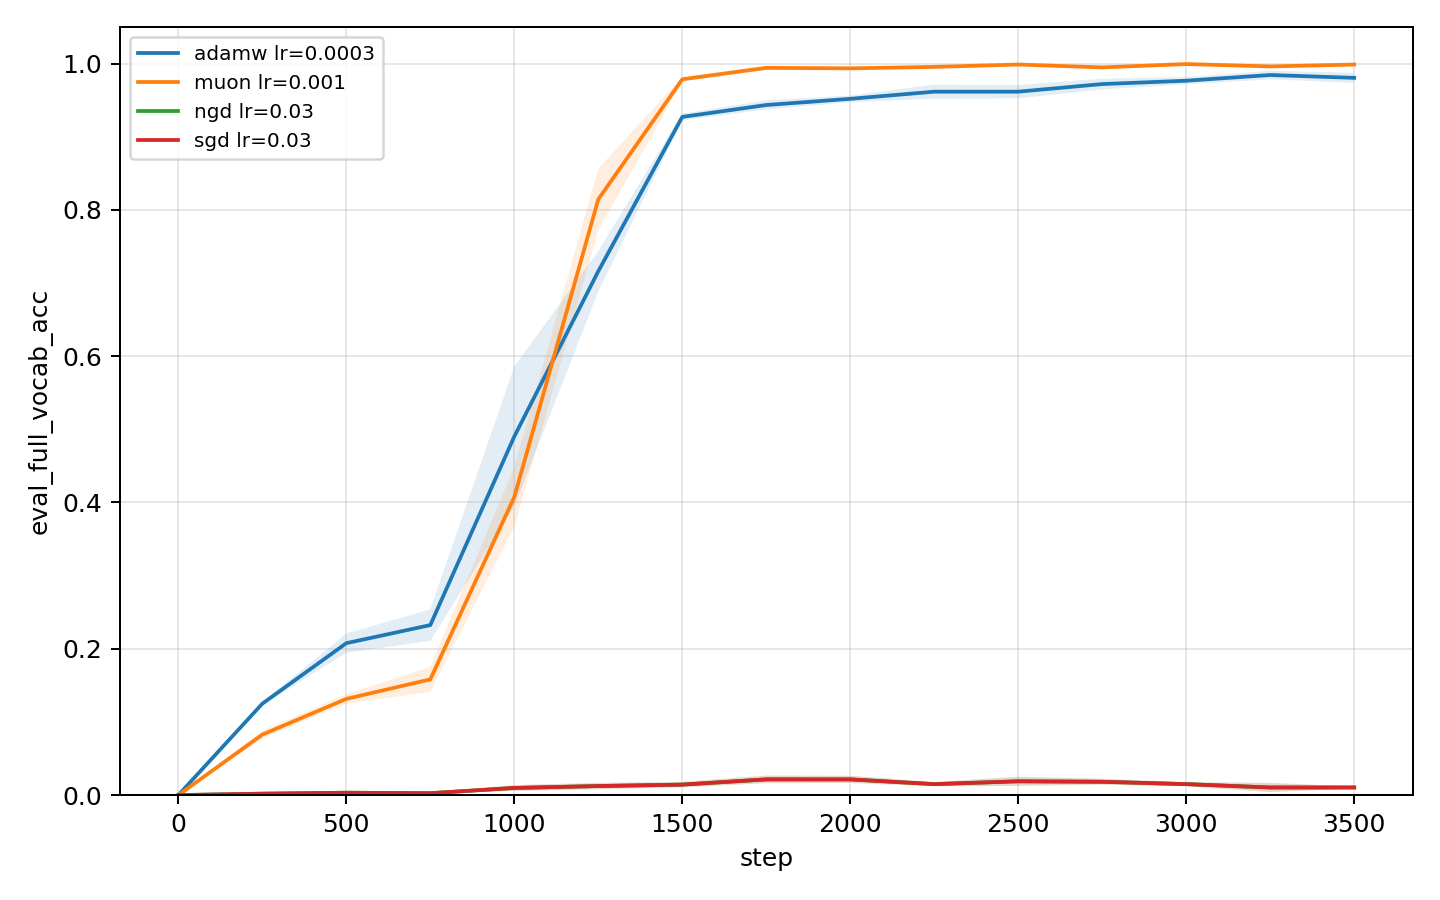
\includegraphics[width=\textwidth]{figures/optimizer_full_vocab_curves_best_lr.png}
  \caption{Full-vocabulary accuracy}
\end{subfigure}
\caption{Optimizer learning curves using each optimizer's best learning rate in the completed clipped sweep.}
\label{fig:opt-curves}
\end{figure}
\begin{figure}[H]
\centering
\begin{subfigure}{0.49\textwidth}
  \centering
  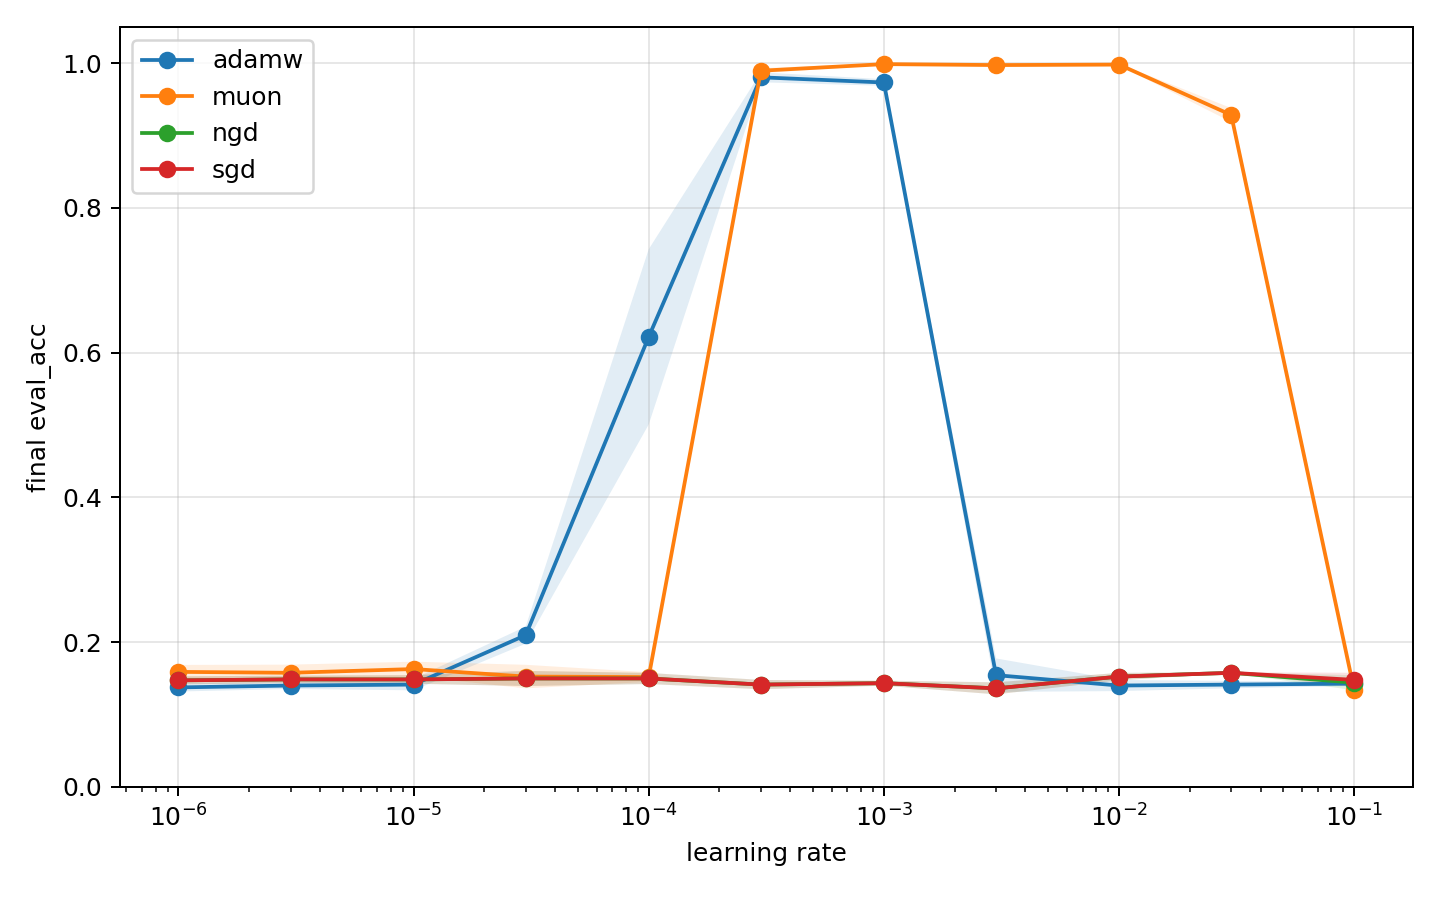
\includegraphics[width=\textwidth]{figures/optimizer_lr_sensitivity.png}
  \caption{Candidate accuracy}
\end{subfigure}
\begin{subfigure}{0.49\textwidth}
  \centering
  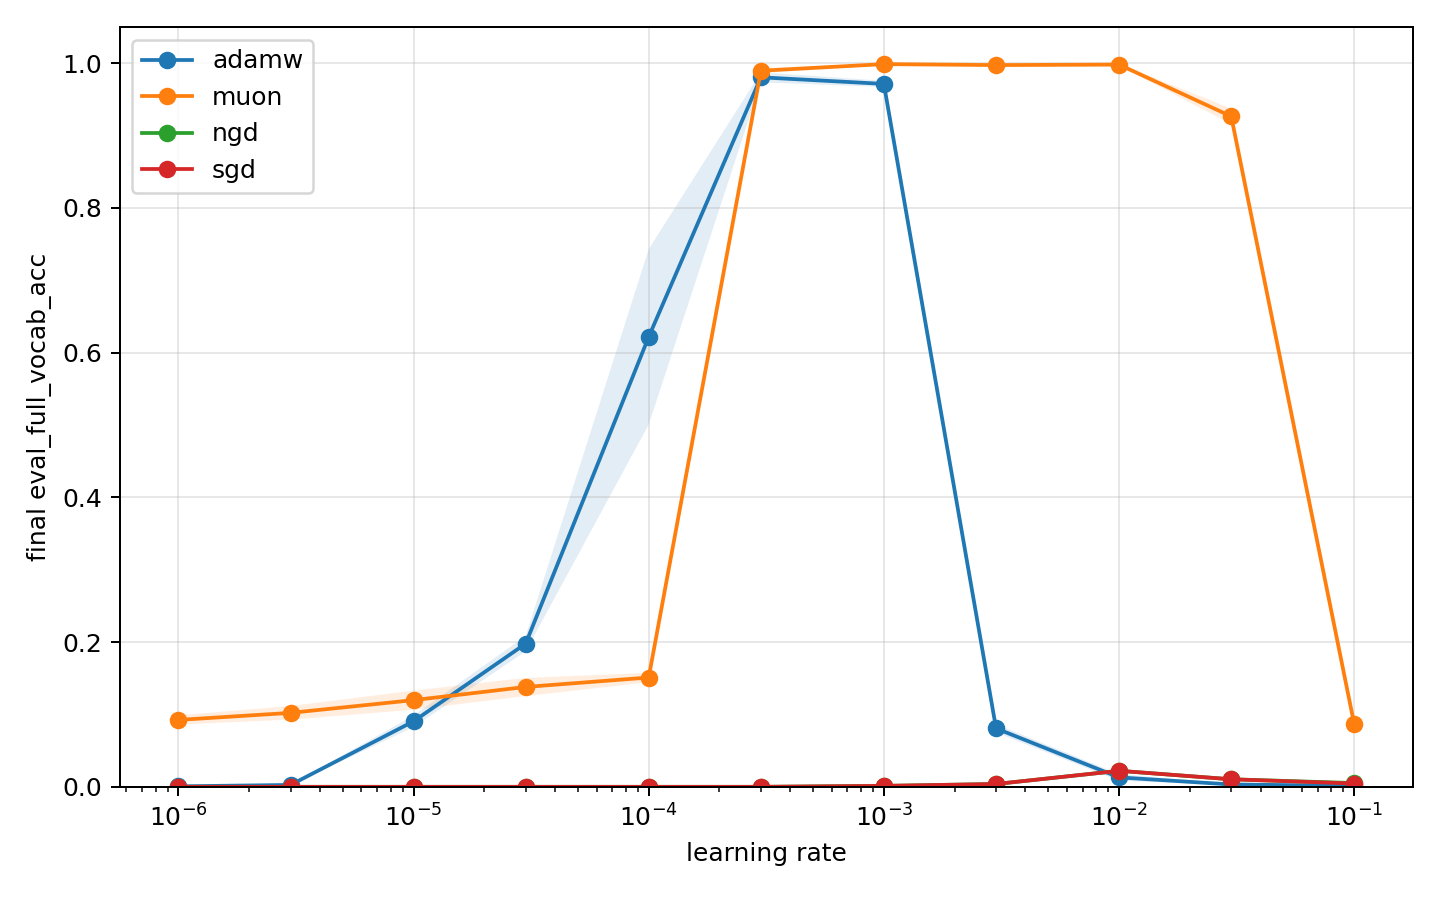
\includegraphics[width=\textwidth]{figures/optimizer_full_vocab_lr_sensitivity.png}
  \caption{Full-vocabulary accuracy}
\end{subfigure}
\caption{Learning-rate sweep across optimizers. Each point is the final evaluation accuracy averaged across seeds for one learning rate; bands show SEM.}
\label{fig:opt-lr-sweep}
\end{figure}

\textbf{Muon has a small advantage over AdamW in this setting, but the task is close to saturated:
AdamW already reaches approximately \(98\%\) accuracy.
Thus the current experiment does not show a large Muon advantage.}
To test for a stronger Muon benefit, the next optimizer study may remove gradient clipping and use harder-but-learnable regimes near the capacity boundary.

\end{document}

